 \documentclass[%
oneside,                 % oneside: electronic viewing, twoside: printing
final,                   % draft: marks overfull hboxes, figures with paths
10pt]{article}

\listfiles               %  print all files needed to compile this document

\usepackage[a4paper, total={6in, 8in}]{geometry}
\usepackage[totoc]{idxlayout}   % for index in the toc
\usepackage[nottoc]{tocbibind}  % for references/bibliography in the toc

\usepackage{relsize,makeidx,color,setspace,amsmath,amsfonts,amssymb}
\usepackage[table]{xcolor}
\usepackage{bm,ltablex,microtype}
\usepackage{comment} 
\usepackage[pdftex]{graphicx}

\usepackage{fancyvrb} % packages needed for verbatim environments

\usepackage[T1]{fontenc}
%\usepackage[latin1]{inputenc}
\usepackage{ucs}
\usepackage[utf8x]{inputenc}

\usepackage{lmodern}         % Latin Modern fonts derived from Computer Modern


\usepackage{pgfplotstable, booktabs}

\pgfplotstableset{
    every head row/.style={before row=\toprule,after row=\midrule},
    every last row/.style={after row=\bottomrule}
}





% Hyperlinks in PDF:
\definecolor{linkcolor}{rgb}{0,0,0.4}
\usepackage{hyperref}
\hypersetup{
    breaklinks=true,
    colorlinks=true,
    linkcolor=linkcolor,
    urlcolor=linkcolor,
    citecolor=black,
    filecolor=black,
    %filecolor=blue,
    pdfmenubar=true,
    pdftoolbar=true,
    bookmarksdepth=3   % Uncomment (and tweak) for PDF bookmarks with more levels than the TOC
    }
%\hyperbaseurl{}   % hyperlinks are relative to this root

\setcounter{tocdepth}{2}  % levels in table of contents

% --- fancyhdr package for fancy headers ---
\usepackage{fancyhdr}
\fancyhf{} % sets both header and footer to nothing
\renewcommand{\headrulewidth}{0pt}
\fancyfoot[LE,RO]{\thepage}
% Ensure copyright on titlepage (article style) and chapter pages (book style)
\fancypagestyle{plain}{
  \fancyhf{}
  \fancyfoot[C]{{\footnotesize \copyright\ 1999-2018, "Computational Physics I FYS3150/FYS4150":"http://www.uio.no/studier/emner/matnat/fys/FYS3150/index-eng.html". Released under CC Attribution-NonCommercial 4.0 license}}
%  \renewcommand{\footrulewidth}{0mm}
  \renewcommand{\headrulewidth}{0mm}
}
% Ensure copyright on titlepages with \thispagestyle{empty}
\fancypagestyle{empty}{
  \fancyhf{}
  \fancyfoot[C]{{ }}
  \renewcommand{\footrulewidth}{0mm}
  \renewcommand{\headrulewidth}{0mm}
}

\pagestyle{fancy}


% prevent orhpans and widows
\clubpenalty = 10000
\widowpenalty = 10000

% --- end of standard preamble for documents ---


% insert custom LaTeX commands...

\raggedbottom
\makeindex
\usepackage[totoc]{idxlayout}   % for index in the toc
\usepackage[nottoc]{tocbibind}  % for references/bibliography in the toc
\usepackage{listings}
\usepackage[normalem]{ulem} 	%for tables
\useunder{\uline}{\ul}{}
\usepackage{hyperref}
\usepackage[section]{placeins} %force figs in section

\usepackage{natbib}

\usepackage[toc,page]{appendix} % appenix


%-------------------- end preamble ----------------------

\begin{document}

% matching end for #ifdef PREAMBLE

\newcommand{\exercisesection}[1]{\subsection*{#1}}


% ------------------- main content ----------------------



% ----------------- title -------------------------

\thispagestyle{empty}

\begin{center}
{\LARGE\bf
\begin{spacing}{1.25}
Classifying wine quality using support vector machines and neural networks
\end{spacing}
}
\end{center}

% ----------------- author(s) -------------------------

\begin{center}
{\bf Johan Nereng}
\end{center}

    \begin{center}
% List of all institutions:
\centerline{{\small Department of Physics, University of Oslo, Norway}}
\end{center}
    
% ----------------- end author(s) -------------------------

% --- begin date ---
\begin{center}
Des 13, 2019
\end{center}
% --- end date ---

\vspace{3cm}
\vspace{3cm}
\begin{abstract}
This project aims to examine a classification approach to support vector machines (SVM) and feed forward neural networks (FFNN) in predicting wine quality. The data set used in training and testing the machine learning methods was a data set of 'Vinho Verde' white whine qualities presented by Cortez et al. in their article \cite{CortezPaulo}. As the results presented in said article indicated better prediction for the majority classes (medium quality wines), and worse prediction on very good or very bad wines, this project uses an adaptive synthetic sampling approach (ADASYN) with the intention of improving minority class prediction. The main findings of this project is that this appears to come at the cost of majority class prediction performance, which was reflected in a decreased accuracy score when ADASYN was applied, from $0.57$ to $0.35$ for the FFNN, and $0.57$ to $0.52$ for the SVM. These accuracy scores are somewhat lower than those presented by Cortez et al.  (FFNN: $59.1$, SVM: $62.4$), but qualitative comparison between confusion matrices still indicated increased minority class prediction quality when using ADASYN.
 
\end{abstract}


\newpage


\textit{\textbf{Author's comments:} As there were no direct specifics on the verbosity or contents of the methods section, I opted to follow the advise of Doctoral Research Fellow Øyvind Sigmundson Schøyen about trying to keeping the report brief and to the point. This has allowed me to explore pandas, keras and tensorflow for the first time, as well as getting some more experience with sklearn and other libraries. I have also tried to adopt a style of writing which makes a clear distinction between my own assessments and opinions, and those of others. Feedback on this would be useful as I am unaccustomed to writing reports in a direct and person language. I found the grid-search for hyper-parameters very challenging, and in hindsight wish that I had spent more time on it earlier on, using a wider range of values - though this would have required additional work. Furthermore, I did not realize that I had forgot to cross validate my results before it was too late with regards to the upcoming exam period, which makes the results less robust. Cortez et al. surprised me with their confusion matrices, which I were unable to make complete sense of as they include all the observations in the data set. It is possible that they have have covered the entire data set with their 5-fold cross validation, but I was unable to deduce this from their paper. Lastly, some of the numbers in the correlation matrices I present are hard to read. An unfortunate accident I would have rectified if my current python environment was not conflicted w.r.t plotting.}
\newpage

\section{Introduction}
In their article \textit{Modeling wine preferences by data mining from physicochemical properties} \cite{CortezPaulo}, Cortez et al. presents the possibility of predicting wine quality using support vector machines (SVM) and [forward feed] neural networks (NN) [FFNN] with a regression approach. Their intention is to examine tools that may possibly support the oenologist's wine evaluation, by predicting quality based on physicochemical measurements (alcohol, sulphates, pH etc.). They claim that building such prediction models may have implications for wine certification, wine producers and even wine consumers. Through their work, they achieved promising results with SVMs, outperforming their neural networks. Their results did however indicate a tendency for these machine learning methods to predict better at the majority classes, which were wines of medium quality, than they did at the minority classes, wines of high or low quality. As a wine consumer, my own assessment is that predicting whether a wine is good or bad may be of more direct use than accurately predicting nuances in mediocrity (\textbf{too flippant?}). Thus in this project, I aim to increase the predictive performance of the two machine learning methods on poor and high quality wines, using the same data set as the one used by Cortez. et al. In order to do so, I have adopted a classification approach to the modeling, using both SVMs and FFNNs for testing out two strategies for improving minority class wine quality prediction. The first strategy is using a weighted F1 score to asses which model parameters are optimal, which is intended to increase the importance of minority classes in model assessment as the metric calculates a score for each class, then averages the results. The second strategy is to use adaptive synthetic sampling approach (ADASYN) in order to generate additional data entries from the under-represented classes (poor and high quality wines).

Initially in this project, I describe \hyperref[data_pp]{the data set} used to train and test the machine learning methods on and sketch out some possible strategies available to address the class imbalance and the steps data pre-processing used in this project. Then, I present the 
\hyperref[evaluation]{metrics used} for evaluation of model performance; F1 score, accuracy and confusion matrices. In the section on  \hyperref[FFNN]{FFNN}s I then describe the basic properties of such neural networks, as well as the over-all implementation scheme used in this project. A similar and brief description of \hyperref[SVM]{SVM}s follows, before I present the \hyperref[results]{results} produced in this project. The project then wraps up with a summary of the \hyperref[conclusions]{conclusions} made with respect to minority class prediction and overall machine learning performance.

In order to write this project paper and the code required to produce the results, I used a variety of tools, including: Python 3.7.5, NumPy \cite{numpy}, Scikit-learn \cite{sklearn}, Keras \cite{keras}, TensorFlow \cite{tensorflow} and Imbalanced-learn \cite{imblearn}, as well as a number of books, web-pages and articles - of which most are listed under 
 \hyperref[refer]{references}. All the code required to reproduce the results may be found on the author's \href{https://github.com/johanere/FYS-STK4155/tree/master/Project3}{github page }.  



\section{Material and methods} \label{Section_Theory}
\subsection{Data set and pre-processing} \label{data_pp}
Cortez et al. \citep{CortezPaulo} used two data sets, one for the white variant and one for the red variant of the Portugeese "Vinho Verde" wine. In order to more easily focus the implementation and analysis of the machine learning methods, and because the data set of red wines is small ($1599$ observations), I chose to only uses the data set of white wines. The data consists of $4898$ observations of $11$ physicochemical measurements such as alcohol, sulphates and pH, collected from samples tested at the CRVV, an inter-professional organization dedicated to 'Vinho Verde' whines in the period 2004-2007 \citep{CortezPaulo}. The data set also includes quality scores of $0$ to $10$, which this project aims to predict, with $0$ being very bad and $10$ excellent, set by a median of three blind tasters. 

The distribution of quality scores in the data set is clearly imbalanced, as well somewhat  skewed (see figure \ref{fig:initial}). Data imbalance such as this is prone to results in training bias towards the majority classes \cite{HaiboHe2008AAss}, and was therefor a problem that needed to be addressed. Commonly, methods used for imbalanced learning problems may be categorized as either sampling strategies, synthetic data generation, cost-sensitive training, active learning, or kernel-based methods \cite{HaiboHe2008AAss} - which are mainly applied to training data. In this project, I opted to use two techniques,  kernel transformations (rbf \citep{MLMurphy}[p.479-483] and polynomial \citep{2002PRwS}[p.243]) and ADASYN \cite{HaiboHe2008AAss}. ADASYN is an adaptive synthetic sampling approach which generates additional samples of the minority class observations that are hardest to learn. This reduces the bias introduced by the imbalanced data, and adjusts the classification decision boundary toward minority classes. In order to more easily compare the results in this project with those of Cortez et al., I split the data as they did; 1/3 test and 2/3 training \citep{CortezPaulo}. However, as ADASYN uses $K$-nearest neighbors in it's data generation  \cite{HaiboHe2008AAss}, a 1/3 and 2/3 split resulted in too few (wine quality) class $9$-neighbors for effective data generation. Due to this, I decided to apply the simple and somewhat crude sampling strategy of deleting all entries with quality $9$ prior to the to test-training split. Looking at Cortez et al. they omitted grade 3 and 9 all together from their evaluation since they never had any predictions in those categories \citep{CortezPaulo}. Instead of training on two categories that are not used, I also opted to remove grade $3$ as well as $9$ from the data prior to pre-processing.  

The pre-processing of the data prior to training in this project was thus: \textbf{1.} Remove all entries of quality $3$ and $9$. \textbf{2.} Split into test (1/3) and training (2/3). \textbf{3.} Use ADASYN to generate additional synthetic training data. \textbf{4.} (Applies to both test and training data) Scale predictors to range $[0,1]$ and one-hot encode targets. \textbf{5.} Apply kernel transformation (only used for SVM).

 
 

\begin{figure}[!h]
        \centering 
         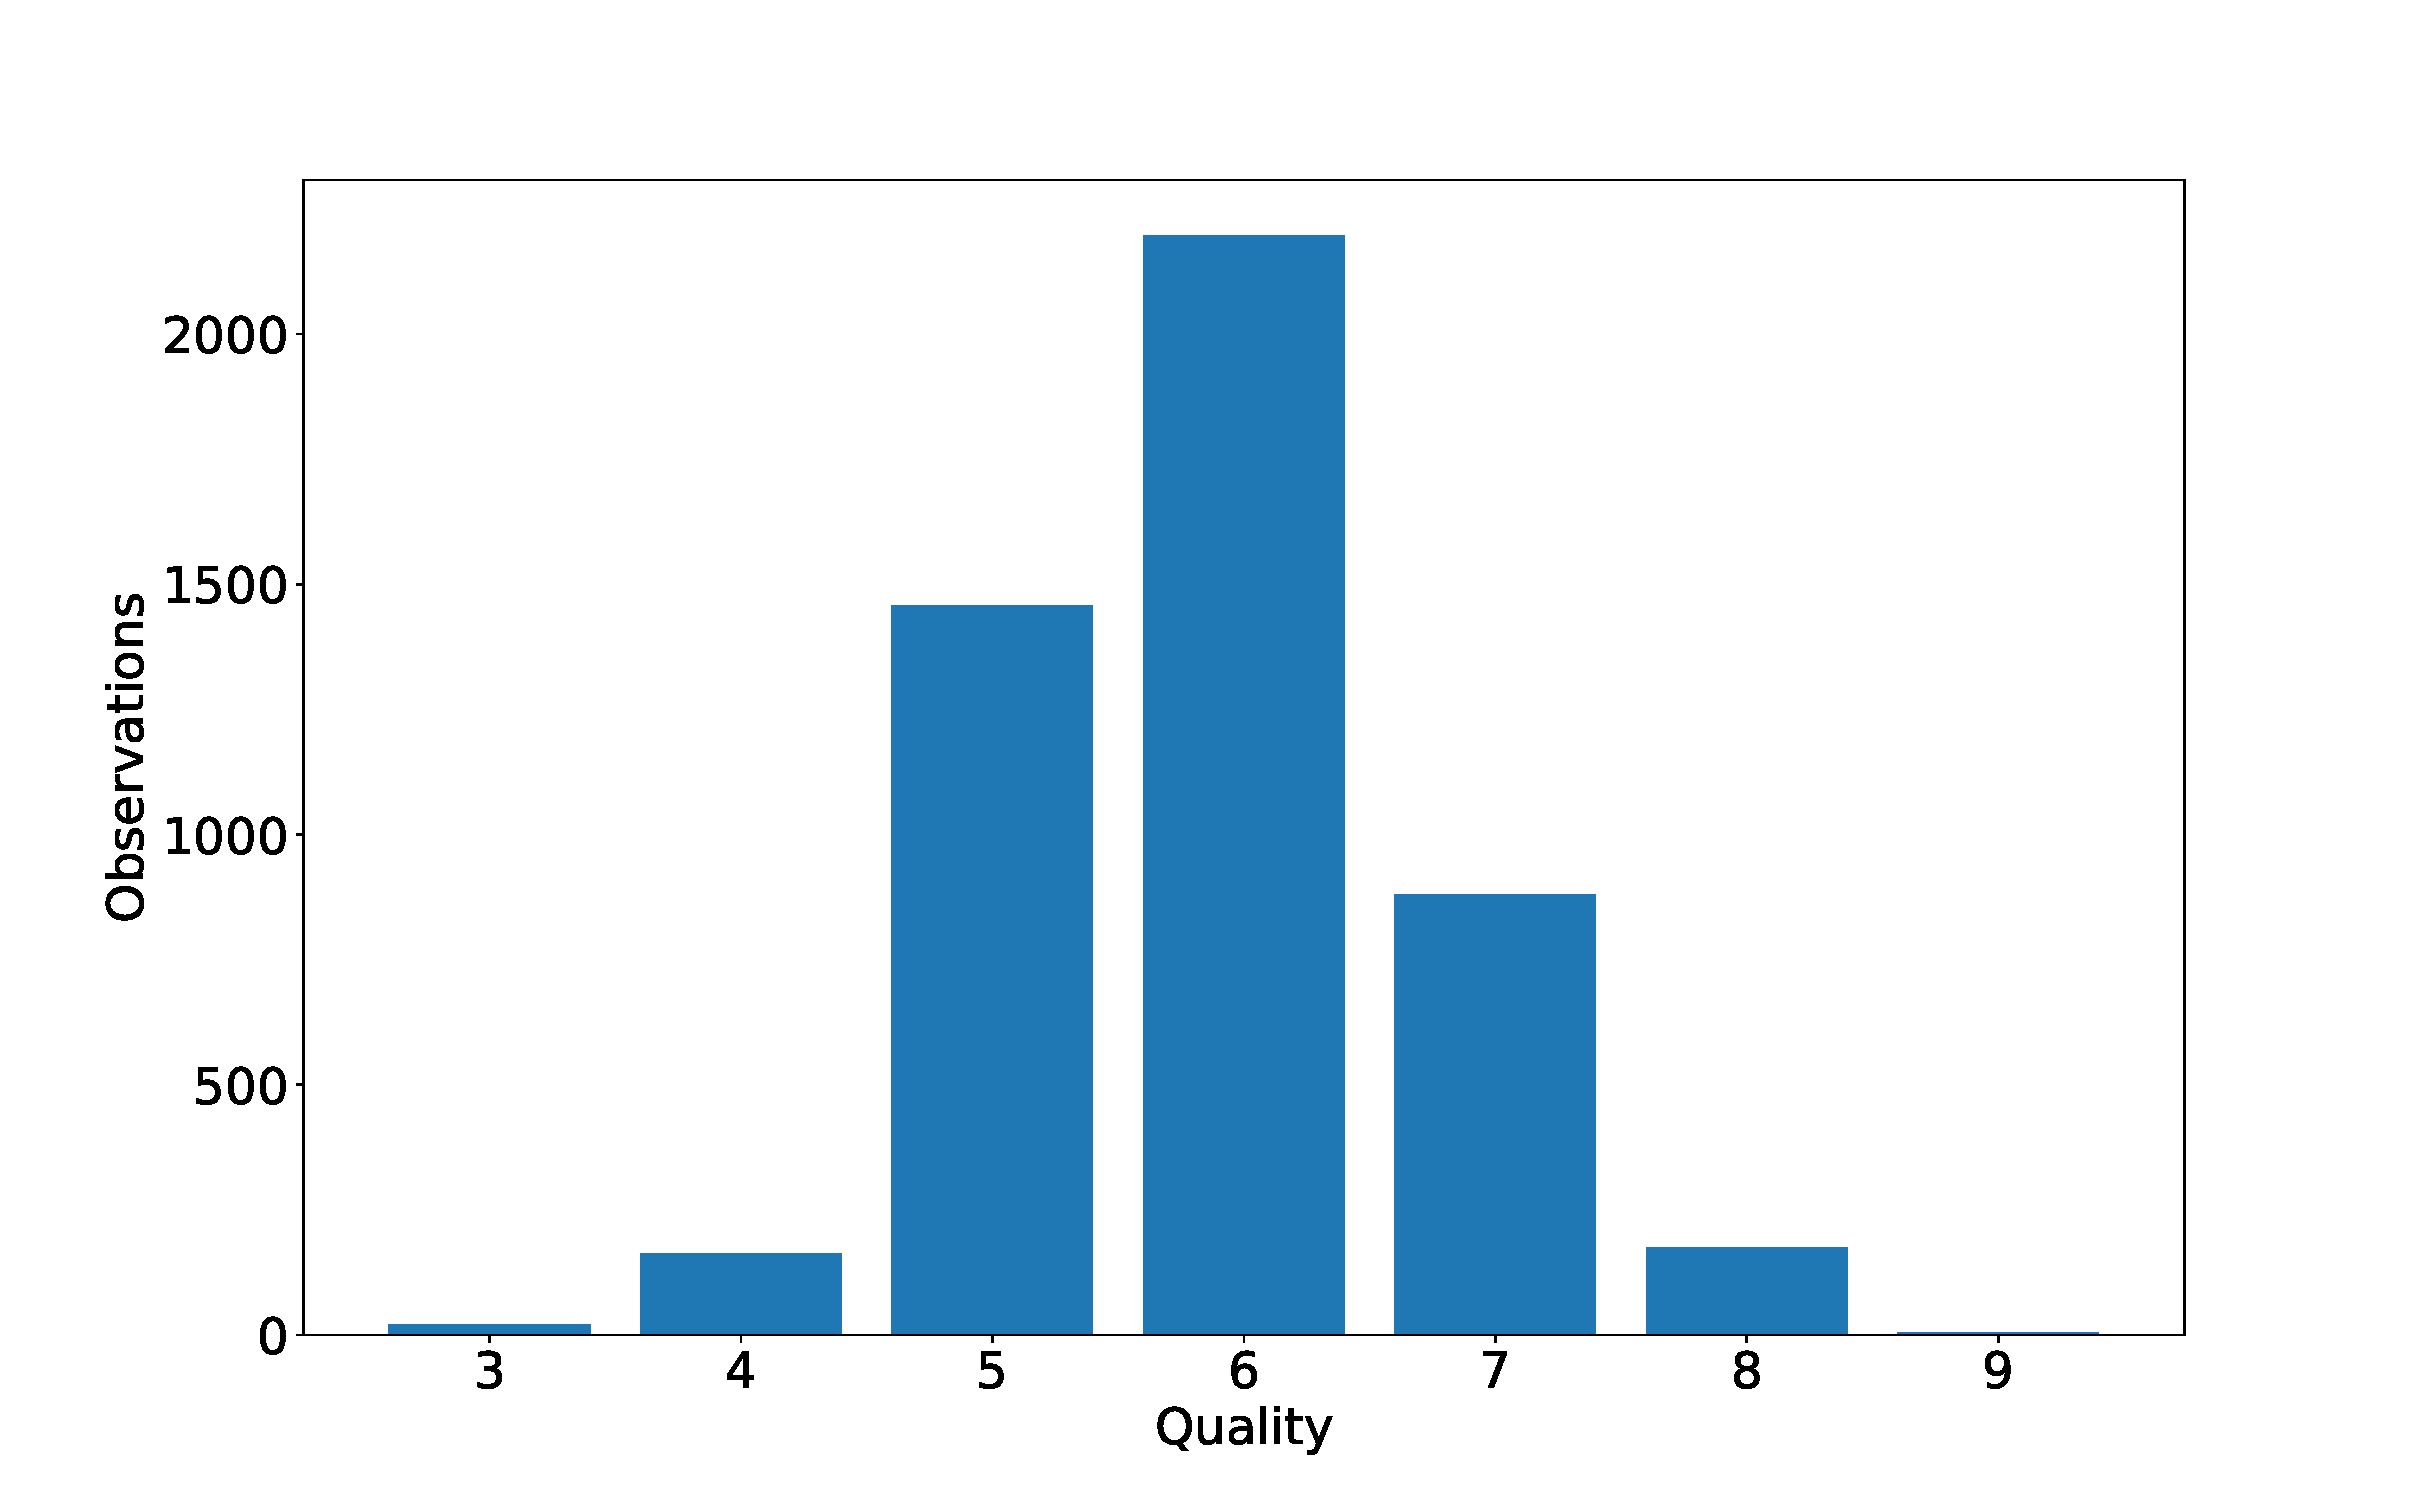
\includegraphics[scale=0.30]{../Results/bar_y.pdf} 
        \caption{Bar plot of quality distributions in white wine data. Corresponding sample numbers are; $20,163,1457,2198,880,175,5$.}
        \label{fig:initial}   
\end{figure}  

\subsection{Supervised learning methods and project implementation} 
Similar to Cortez et al. this project uses feed forward neural networks (FFNN), also known as multi-layer perceptron models (MLP), and support vector machines (SVM). As both methods were implemented with the use of a variety of hyper parameters governing their structure and performance, I used grid-searches to iterate permutations of the applied hyper parameters pertaining to each method in order to find the 'optimal' (depending on choice estimator) combination of values. 

\subsection{Evaluation and performance measurements} \label{evaluation}
In order to compare results to some degree with Cortez et al. this project evaluates it's learning methods with accuracy score (not sensitive to data imbalance), corresponding to accuracy with tolerance $T=0.5$ used by Cortez et al.,  and qualitative examination of confusion matrices. As an example, figure \ref{fig:confusion} shows a confusion matrix with true positives (TP), false positives (FP) and false negatives (FN) for category $3$.  Cortez et al. also evaluates their methods with mean average deviation (MAD) \citep{CortezPaulo} - however, as this project makes a classification approach, MAD is less suited. Instead, F1 score \eqref{eq:F1} is used, which is a combined measurement of precision and recall \citep{MLMurphy}[p.183]. When estimating the 'optimal' hyper-parameter combination, I opted to use a macro-average (calculates metric independently for each class, then averages) of the F1 score when using ADASYN. When not using ADASYN, I chose to use the weighted F1 score (weighted average of class scores) as scoring metric instead, as the weights some extent may address the bias from the imbalanced data set. As a performance scoring metric (on test data), F1 (weighted) is used, as the training data is guaranteed to be unbalanced due to the stratified split of the original data. In order to maintain some quantitative basis for comparison with Cortez et al. I also opted to keep the accuracy score as a metric, even though it is not well suited for imbalanced data sets.
\begin{equation}
F1=2 \frac{ precision * recall}{precission + recall}
\label{eq:F1}
\end{equation}
Where $recall = \frac{\text{true positives}}{\text{true positives} + \text{false negatives}} $, and $precision = \frac{\text{true positives}}{\text{true positives} + \text{false positives}} $, for a given class.


\begin{figure}[!h]
        \centering 
         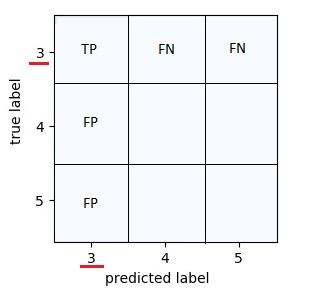
\includegraphics[scale=0.8]{confusion.jpg} 
        \caption{A confusion matrix showing true positives (TP), false positives (FP) and false negatives (FN) for category $3$.}
        \label{fig:confusion}   
\end{figure}  
\subsubsection{FFNN} \label{FFNN}
The FFNN is a serial network of ordered regression models (neurons) with connected inputs and outputs \citep{MLMurphy}[p.563]. The neurons are structured in layers, where each layer consists of a number of neurons which use the outputs of the previous layer as their input. The number of  hidden layers of neurons (layers other than first and last layer) is directly associated with the complexity the network is able to approximate. With one hidden layer, the network is typically able to approximate mappings from one finite space to another. Increasing the number hidden layers to two may normally allow representations of arbitrary decision boundaries to arbitrary accuracy (with some caveats, such as function smoothness) \cite{layers}, making such networks universal approximators \citep{MLMurphy}[p.564]. More than two layers may facilitate learning behavior akin to automatic feature engineering. The number of neurons in each (hidden) layer is also closely connect to the approximation ability of the network. Too many neurons may result in over-fitting, while too few may results in under-fitting.

 In this project, I used the rules-of-thumb presented by J.Heathon on NN structures  \cite{layers}; fixing the input layer to to $11$ neurons (corresponding to the number of predictors) and the output layer to $5$ neurons (corresponding to the qualities $4,5,6,7,8$). The choice between one and two hidden layers were left to grid-search optimization along with the number of neurons in these hidden layers (6,7, or 8). For the training regime of the network, I chose to use the ADAM method \citep{adam}, a fast and robust stochastic optimizer which require little tuning. ADAM uses regularization parameters for the first and second moments of the gradient, $\beta_1$ and $\beta_2$. 
 
The neural network was implemented using the Scikit-Learn classifier interface from Keras, which enabled Scikit-learn grid-search with cross validation. The search was carried out on the learning rate of the ADAM optimizer, the decay, activation function of the neurons (final layer fixed with categorical crossentropy), dropout, epochs and batch sizes, using   F1 (weighted or mean) as scoring. The remaining hyper-parameters were set to standard values (such as ($\beta_1=0.9$ and $\beta_2=0.99$), thus focusing on narrowing down the range of values of the parameters that usually have a wider range (such as epochs, batch size and learning rate). The correlation matrices of these grid-searches were then studied together with epoch-wise printing of cost function values, before moving on to repeated runs with variations on the entire hyper-parameter specter. An example of the hyper-parameter correlation matrix used in the initial narrowing down of FFNN  parameter values is shown in figure \ref{fig:corr_parameters} in  \hyperref[APP_1]{appendix 1}, indicating that lower values of epochs and higher learning rate will tend to increase F1 score.

\subsubsection{SVM} \label{SVM}
Unlike FFNN, SVM is a non-probabilistic approach to classification. Instead of training a method in the manner that neural networks do, SVM finds a hyper-plane in feature space. This hyper-plane separates the targets with the optimal margin between categories, providing a unique solution \citep{HastieTrevor2009TEoS}[p.132]. In most cases, the feature space of a problem requires a kernel transformation in order to effectively separate the classes. As such, the specific kernel transformation applied is crucial for which hyper-plane the SVM ends up producing. SVM also relies on a regularization parameter, C, which regulates the margin of separation in finding the  optimal hyper-plane - higher values of C will tend to result in a smaller separation margin in order to correctly classify more samples. In contrast, the shrinkage parameter controls whether or not to allow breaches in margin at all.
	
In this project, I chose to use a radial basis function, or rbf kernel \eqref{eq:rbf} \citep{2002PRwS}[p.243], and polynomial kernel transformation \eqref{eq:rbf} \citep{MLMurphy}[p.482]. The SVM is implemented using Scikit-learn's SVC method, and grid-searching for hyper parameters similar to the FFNN's search, is used on kernel transformation, C, and regularization coefficient.
\begin{equation}
\kappa(\bm x, \bm x') = exp(-\frac{||\bm x - \bm x'||^2}{2 \sigma^2})
\label{eq:rbf}
\end{equation}
\begin{equation}
\kappa(\bm x, \bm x') = (<\bm x^T \bm x'> +c)^d
\label{linear}
\end{equation}
Where $\bm x, \bm x'$ are two objects in some abstract space, $\sigma^2$ the bandwidth \citep{MLMurphy}[p.479-p.480], $c$ a free parameter, and $d$ the degree of the polynomial.



\section{Results} \label{Section_Results} \label{results}
\begin{figure}[!h]
        \centering 
         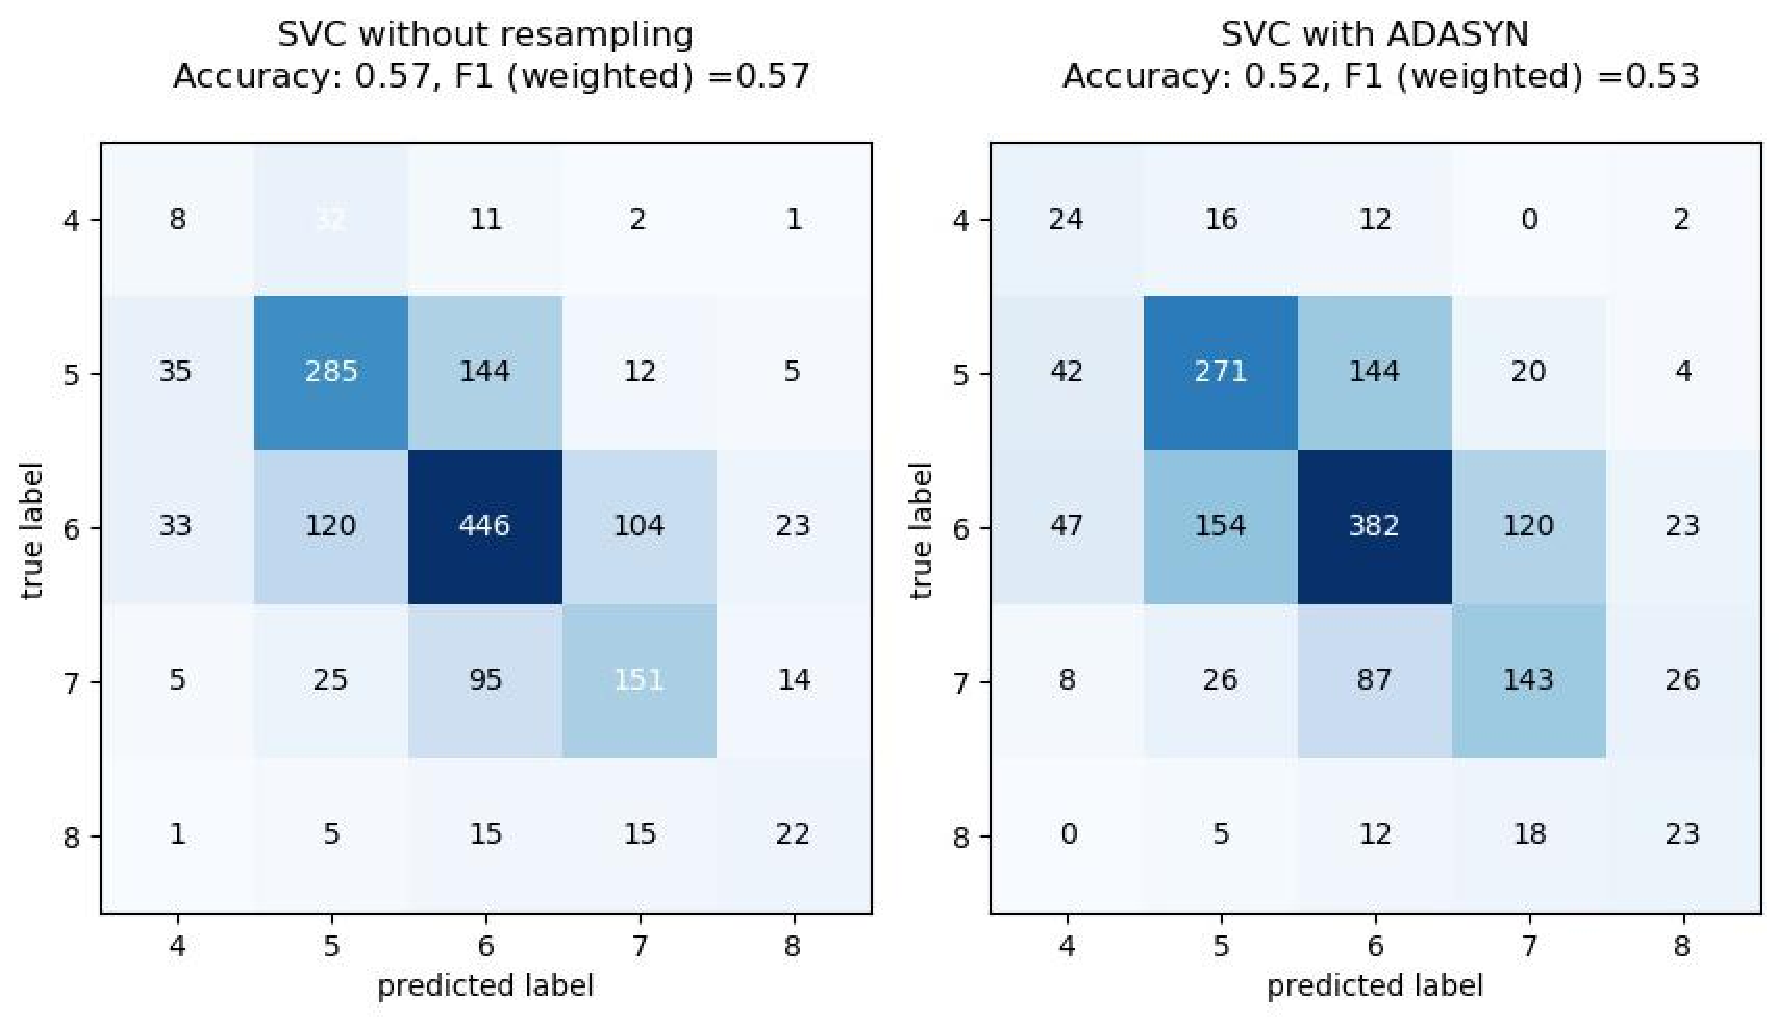
\includegraphics[scale=0.5]{../Results/confusions_SVM.pdf} 
        \caption{Confusion matrices for the SVM on training data, with and without ADASYN}
        \label{fig:conf_SVM}   
\end{figure}  
The 'optimal' hyper-parameter combination suggested using a degree 10 polynomial kernel with a large regularization parameter ($C=1$) and a large coefficient ($c =0.8$ and $1$).
Without any adjustment, these initial SVM hyper-parameters were then used to 'train' the SVM on training data (2/3 of the data) with and without ADASYN. The subsequent prediction performances on the remaining 1/3 of the data in terms of accuracy score, F1 (weighted) score and correlation matrix, are shown in figure \ref{fig:conf_SVM}. In the case of no re-sampling, the SVM accuracy score ($0.57$) is somewhat lower than the SVM performance presented in their paper ($62.4 \pm 0.4$)\citep{CortezPaulo}. The number of FPs from quality $4$, and $8$ present in both confusion matrices (no re-sampling and ADASYN) indicate an increased minority class focus when compared with the SVM confusion matrix from Cortez et al.(figure 3. \citep{CortezPaulo}). This may be the result of having used F1 (weighted) in determining hyper-parameter combination. For quality $4$, $TP<FN$, which may indicate that the hyper-plane is not properly adjusted towards the minority class, despite having a significantly larger decision area for that class. The same trend is seen for quality $8$, but to a less extend, where $TP\sim$ class-wise $FN$. Directly comparing numbers with the confusion matrix from Cortez et al. is not feasible, as their confusion matrix (figure 3. \citep{CortezPaulo}) appears to include all $4898$ observations in the data set. It is unclear to me if this means that they are doing performance evaluation on the the entire data or not. 

For the SVC with ADASYN, the accuracy ($0.52$) and F1 (weighted) ($0.53$) is less than for the SVC with ADASYN. The number of $TP$s for qualities $4$ (the smallest minority class), is however substantially higher, as well as the general miss-classification of qualities far from the true quality. In the SVM confusion matrix of Cortez et al. the miss-classifications are smaller still, but the ratio of $TP$ to $FP$ for class $4$ is a lot lower.

In the case of the FFNN, the performance on test data with hyper-parameter combination from the grid-search is presented in figure \ref{fig:conf_grid}. Without re-sampling, the FFNN accuracy score ($0.57$) is similar to the NN performance presented in their paper ($59.1 \pm 0.3$) \citep{CortezPaulo}. Judging by the correlation matrix, the FFNN without re-sampling favors the majority class $5$, and to some lesser extend $4$ and $6$, without being able to predict any qualities of $3$ and $7$. This is a stark contrast to SVM performance using grid-search hyper-parameter combination, which predicted on all $5$ classes.  The FFNN with ADASYN has an accuracy of $0.003$, and judging by the correlation matrix, does not seem to have achieved any learning with the grid-search hyper-parameters. Due to the initial performance of the FFNN using ADASYN, the hyper-parameters were re-adjusted in an iterative process, resulting in the performance presented in figure \ref{fig:conf_NN}. These results were obtained after increasing epochs from $8$ to $20$, re-adjusting batch-size to $50$ (from $10$ without re-sampling and $200$ with ADASYN), decreasing in dropout ($0.1$ to $0.03$), and adding a second hidden layer. Comparing figures \ref{fig:conf_grid} and \ref{fig:conf_grid}, these hyper-parameter adjustments appear to only have affected the FFNN with ADASYN, suggesting that a higher sensitivity to hyper-parameter tuning for FFNNs when combined with ADASYN.

\begin{figure}[!h]
        \centering 
         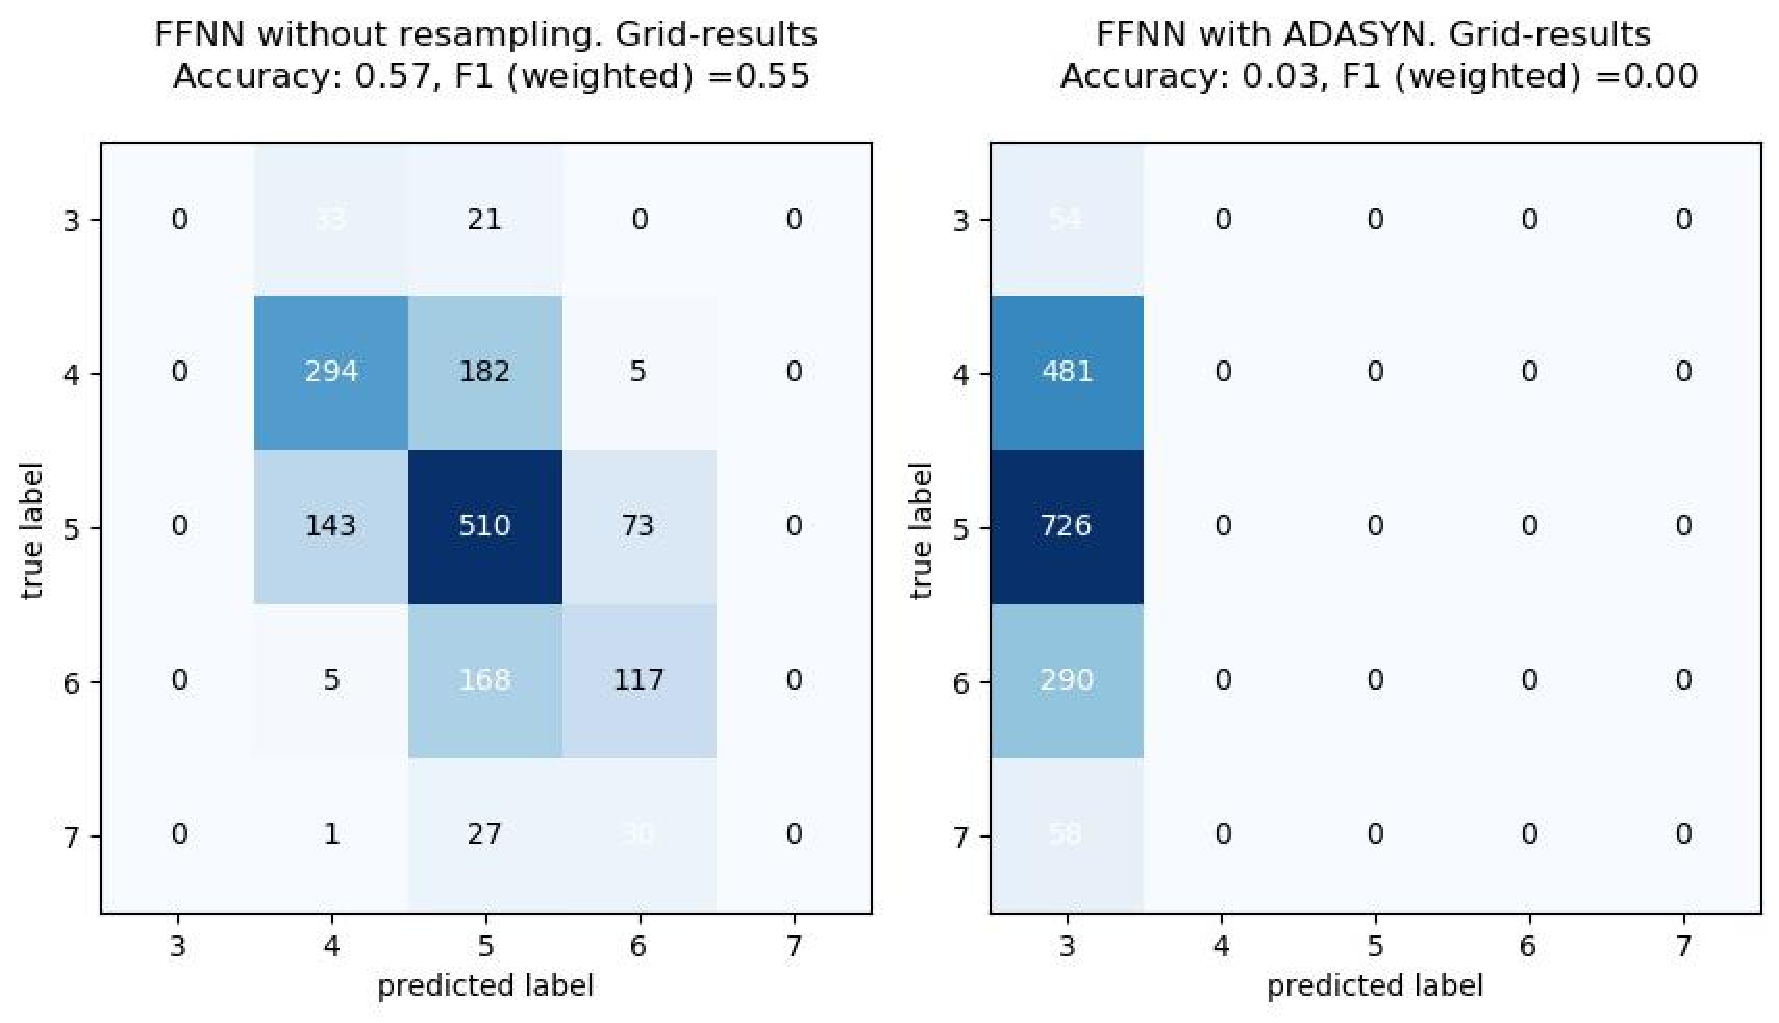
\includegraphics[scale=0.5]{../Results/confusions_NN_grid.pdf} 
          \caption{Confusion matrices for the FFNN on training data, with and without ADASYN, using grid-search hyper parameters}
        \label{fig:conf_grid}   
\end{figure}  

The FFNN with ADASYN after hyper-parameter tuning has a lower accuracy ($0.35$) and F1 score ($0.38$) than the FFNN without re-sampling and SVM, both with and without ADASYN. The number of $FN$ for minority classes is however significantly lower, and the number of $TP$ for minority classes higher. The network does however produce a very large number of 
$FN$s for the majority classes. As the hyper-parameter adjustment included adding another hidden layer, it is possible that the improvement on minority class prediction may prescribed to this added complexity of the data set. After having tested further tweaking of hyper-parameters, including increasing epochs to the thousands, and batch-size up to one thousand, the trade-off between majority and minority classes persist. 



\begin{figure}[!h]
        \centering 
         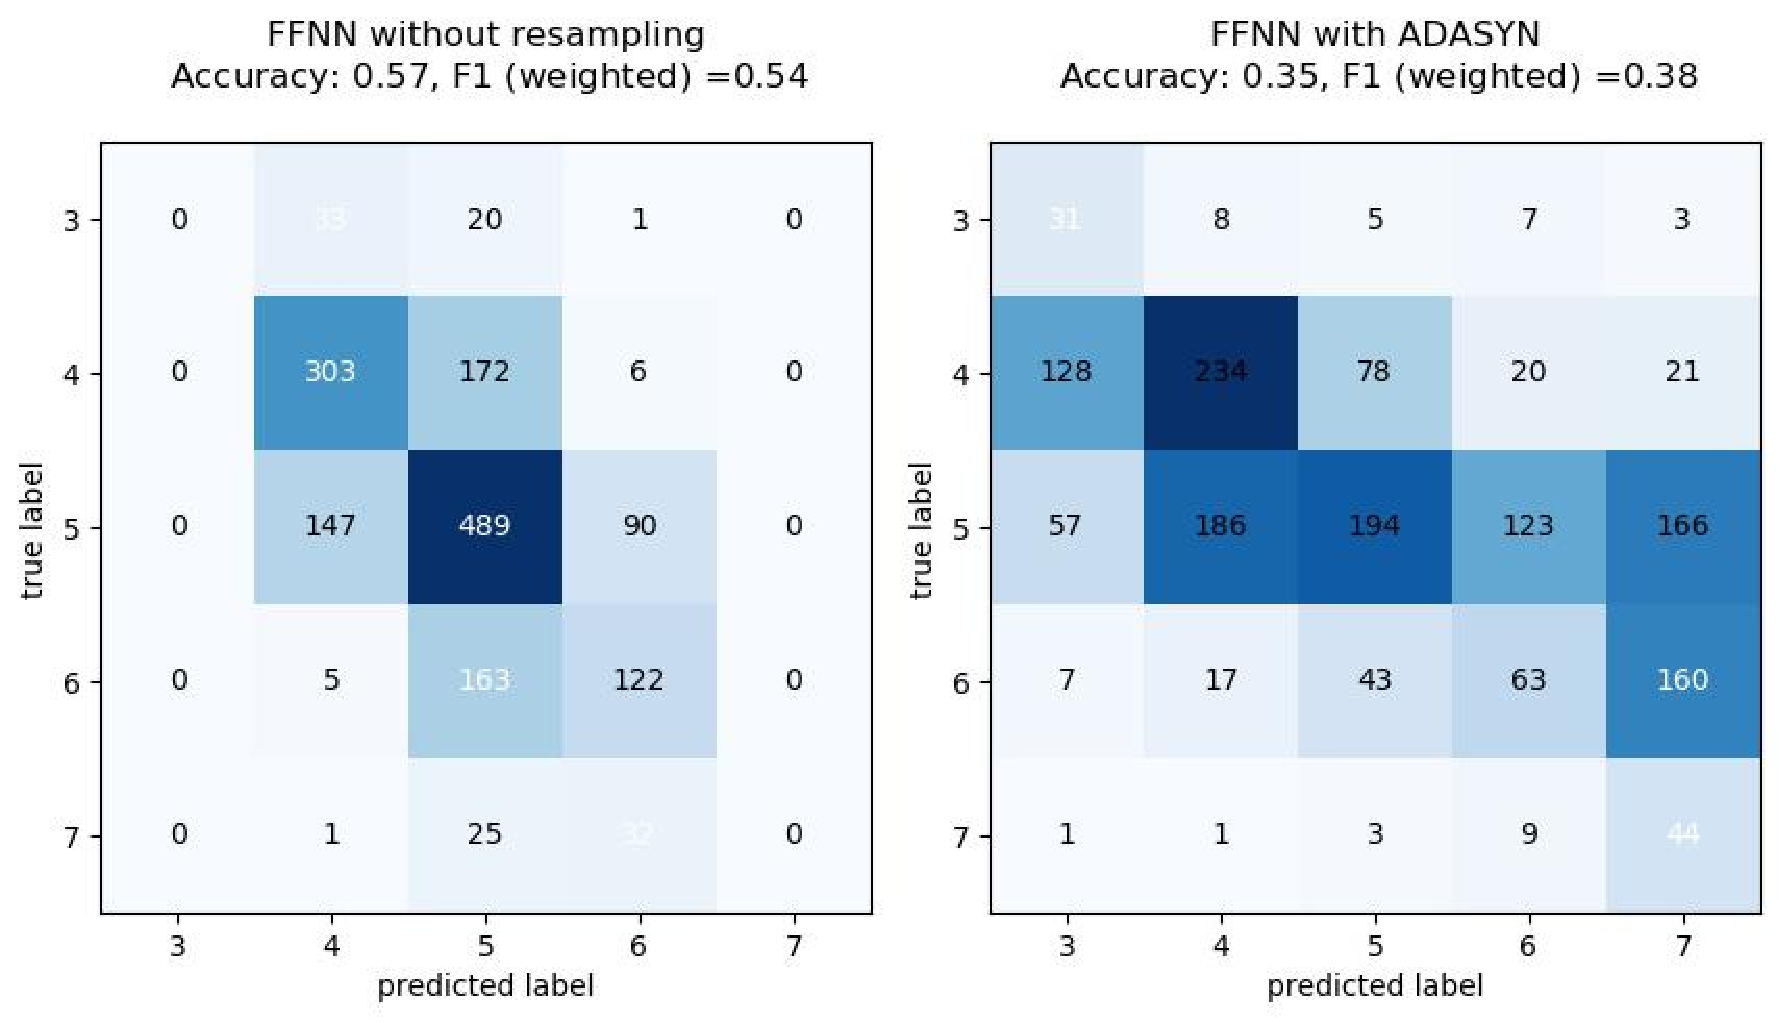
\includegraphics[scale=0.5]{../Results/confusions_NN.pdf} 
          \caption{Confusion matrices for the FFNN on training data, with and without ADASYN}
        \label{fig:conf_NN}   
\end{figure}  
\textit{Cross validation was only used in the hyper-parameter grid-searches, and not in producing the results presented here. This constitutes a discrepancy in the reliably of the presented measurements.}
As the all the F1 scores recorded in the results presented in this project are close to the recorded accuracy scores, and vary the same from model to model, accuracy scores are chosen to be included in the below conclusions instead of F1 scores. This enables a closer comparison with the results from Cortez et al.'s article, as they did not include F1 scores.

\section{Conclusions} \label{conclusions}
Based on the results produced in this project, I conclude that the application of an adaptive synthetic sampling approach (ADASYN) results in improved performance for both support vector machines (SVM) and feed forward neural networks (FFNN) in predicting wine quality among minority classes from unbalanced data. The results produced in in this project also indicates that the improved minority class prediction comes at the cost of majority class prediction performance, which is reflected in a decreased accuracy score from $0.57$ to $0.35$ for the FFNN, and $0.57$ to $0.52$ in the case of the SVM - keeping in mind that accuracy is not well suited for unbalanced data. The evaluated FFNNs performed better at minority class prediction than the SVMs, but had significantly worse accuracy score with ADASYN. Comparison of the results to those of Cortez et al. \citep{CortezPaulo} strengthens the observations on majority vs minority prediction quality. Results from the same paper also suggests that a regression reproach (accuracy NN: $59.1$, SVM: $62.4$) is preferable to a classification approach for predictions on the 'Vinho Verde' data set when synthetic re-sampling is not used. However, as Cortez. et al has not utilized synthetic re-sampling, I am unable to make any decisive conclusions on the observed improved performance on minority class prediction with respect to a classification vs regression approach. Further research including grid-searches with a wider range of hyper-parameters than those used in this project may yield better results on majority class prediction for classification approaches with ADASYN, and could be carried out with access to more powerful computers. 



\bibliography{ref} \label{refer}
\bibliographystyle{plain}


\begin{appendices}
\section*{Appendix 1.} \label{APP_1}
\begin{figure}[!h]
        \centering 
         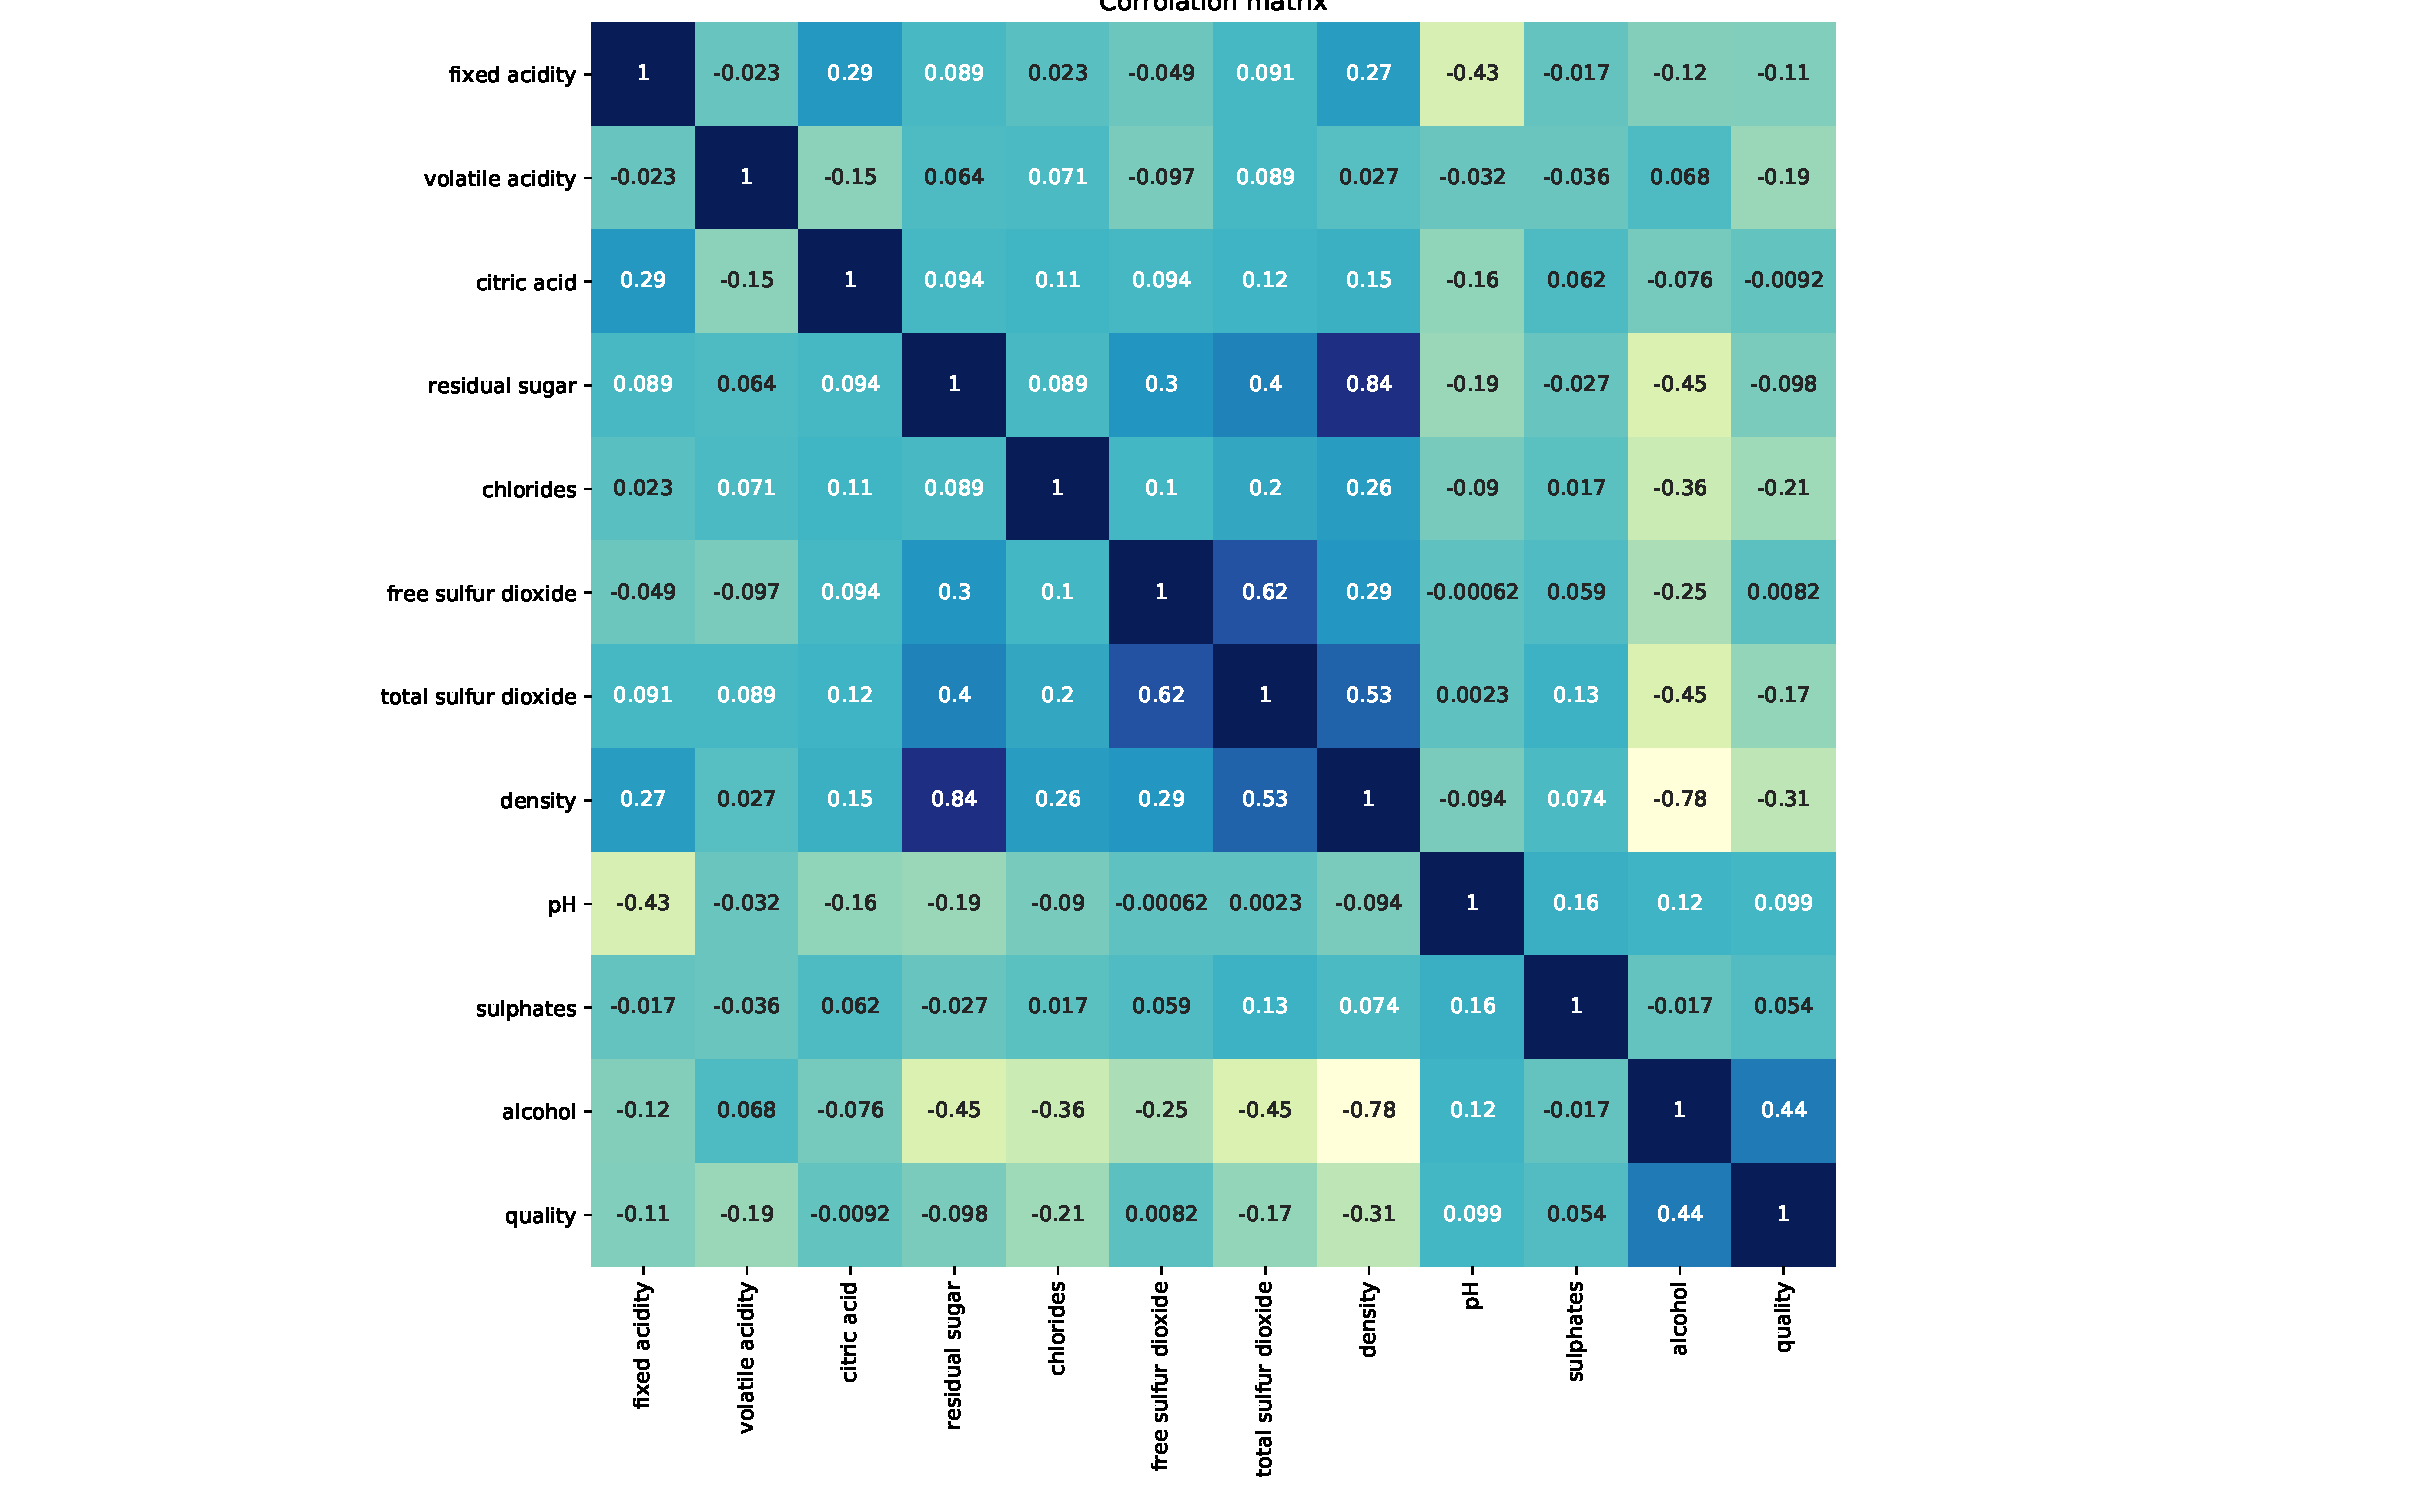
\includegraphics[scale=0.45]{../Results/corrolation_X.pdf} 
        \caption{Corrolation matrix for data set of whine wines}
        \label{fig:corr_parameters}   
\end{figure}  

\begin{figure}[!h]
        \centering 
         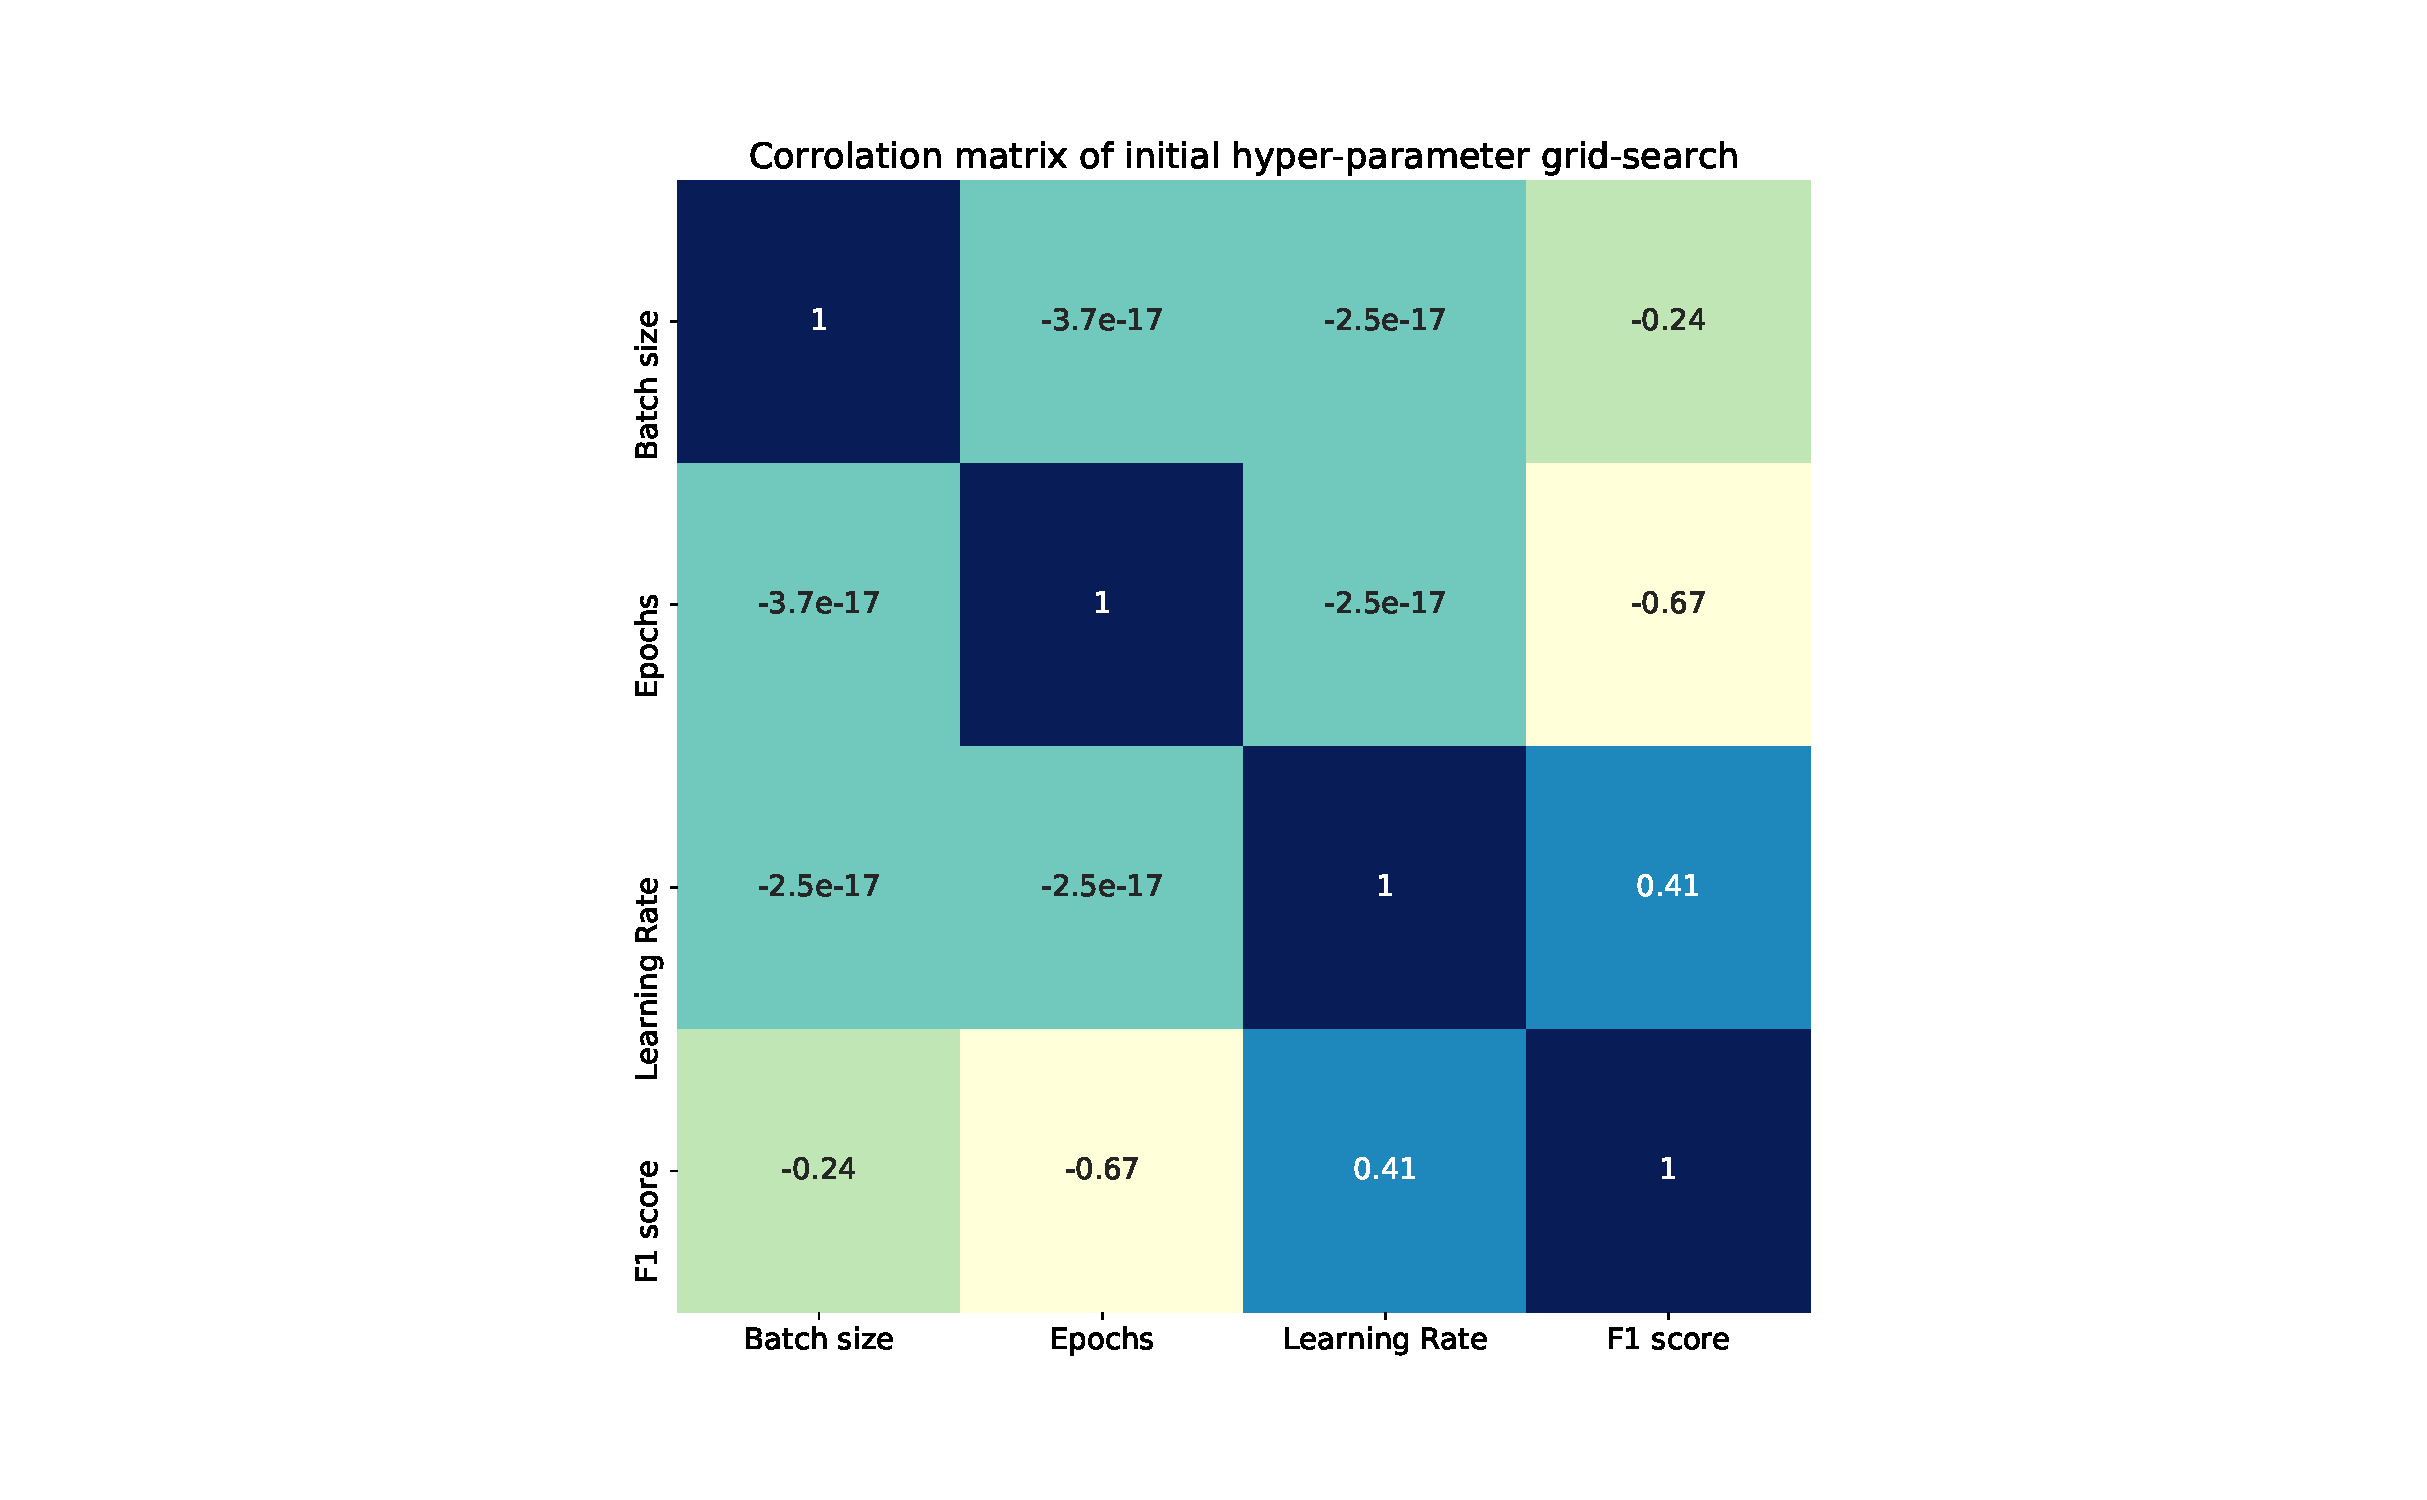
\includegraphics[scale=0.4]{../Results/inital_hyperparam.pdf} 
        \caption{Corrolation matrix initial hyper-parameter search}
        \label{fig:corr_initial}   
\end{figure}  

\end{appendices}
\end{document}